\documentclass[aspectratio=169,11pt]{beamer}

% Theme and color scheme
\usetheme{Madrid}
\usecolortheme{default}

% Packages
\usepackage[utf8]{inputenc}
\usepackage[T1]{fontenc}
\usepackage{graphicx}
\usepackage{hyperref}
\usepackage{listings}
\usepackage{xcolor}
\usepackage{tikz}
\usepackage{array}
\usepackage{booktabs}

% Define colors
\definecolor{utblue}{RGB}{0, 51, 102}
\definecolor{utgray}{RGB}{128, 128, 128}

% Set theme colors
\setbeamercolor{structure}{fg=utblue}
\setbeamercolor{title}{fg=white}

% Title page information
\title{State Registry Data Access Notifications for Estonian eID Holders}
\subtitle{Bachelor's Thesis Defense}
\author{Arkadi Statsenko}
\institute{University of Tartu\\Computer Science Curriculum}
\date{August 2025}

% Footer
\setbeamertemplate{footline}[frame number]

% Remove navigation symbols
\setbeamertemplate{navigation symbols}{}

\begin{document}

% Title slide
\begin{frame}
\titlepage
\begin{center}
\small
Supervisor: Daniel Würsch, MSc
\end{center}
\end{frame}

% Table of contents
% \begin{frame}
% \frametitle{Outline}
% \tableofcontents
% \end{frame}

\section{Introduction}

\begin{frame}
\frametitle{The Problem}
\begin{itemize}
    \item Estonia has numerous state databases containing personal data
    \begin{itemize}
        \item Population Registry (\textit{Rahvastikuregister})
        \item Health Portal (\textit{Terviseportaal})
        \item Digital Registry (\textit{Digiregistratuur})
        \item And many others...
    \end{itemize}
    \item Data is accessed by various parties, including private entities.
    \item {\textit{Andmejälgija} (Data Tracker) exists where users can see data access logs}.
    \item Current system requires manual checking on \textit{eesti.ee}
\end{itemize}

\vspace{0.5cm}
\begin{center}
\textbf{Goal:} Create real-time notifications for data access events
\end{center}
\end{frame}

\section{Background}

\begin{frame}
\frametitle{Current System: \textit{Andmejälgija} (Data Tracker)}
\begin{columns}
\begin{column}{0.3\textwidth}
\begin{itemize}
    \item Protocol created by RIA in 2017
    \item X-Road based distributed system
    \item Users access via \textit{eesti.ee} web portal
\end{itemize}
\end{column}
\begin{column}{0.7\textwidth}
\begin{center}
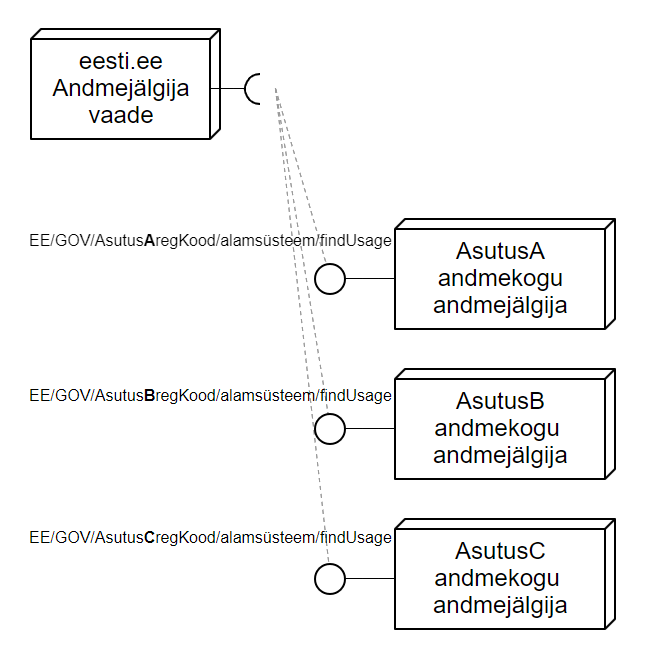
\includegraphics[width=\textwidth]{../english/figures/aj_model.PNG}
\end{center}
\end{column}
\end{columns}
\end{frame}

\section{Implementation Approach}

\begin{frame}
\frametitle{X-Road vs Standalone Approach}
\begin{columns}[t]
\begin{column}{0.47\textwidth}
\begin{block}{X-Road Service}
\textbf{Advantages:}
\begin{itemize}
    \item Full API access to \textit{Andmejälgija}
    \item Multiple potential notification channels
    \item Official integration path
\end{itemize}

\textbf{Disadvantages:}
\begin{itemize}
    \item Legal entity required
    \item HSM hardware (\textasciitilde€9,000)
    \item Compliance obligations
    \item Permission (contract) needed from each data controller
    \item Another data controller introduced
\end{itemize}
\end{block}
\end{column}
\begin{column}{0.47\textwidth}
\begin{block}{Standalone Approach}
\textbf{Advantages:}
\begin{itemize}
    \item No legal entity requirements
    \item Open source development possible
    \item User maintains control
\end{itemize}

\textbf{Disadvantages:}
\begin{itemize}
    \item Reverse engineering of \textit{eesti.ee}
    \item Self-hosting required
    \item Session management complexity
\end{itemize}
\end{block}
\end{column}
\end{columns}
\end{frame}

\begin{frame}
\frametitle{Mobile App: Making Standalone Viable}
\begin{block}{How Mobile App Solves Standalone Limitations}
\begin{itemize}
    \item \textbf{Easy Setup:} One-click installation from GitHub releases
    \item \textbf{Built-in Notifications:} Native Android notification system
    \item Operates as standalone client - no reliance on third-parties.
\end{itemize}
\end{block}

\begin{center}
\textbf{Mobile app transforms standalone approach into a practical solution}
\end{center}
\end{frame}

\section{Technical Solution}

\begin{frame}
\frametitle{Data Access Notifier - Architecture}

\begin{columns}[t]
\begin{column}{0.40\textwidth}
\begin{itemize}
    \item Authentication to \textit{eesti.ee} happens through TARA, leveraging Android WebView.
    \item Resulting cookies are used to poll internal \textit{eesti.ee} API
    \item A combination of AlarmManager and foreground services is used for consistent session extention and API polling.

\end{itemize}
\end{column}

\begin{column}{0.60\textwidth}
\begin{center}
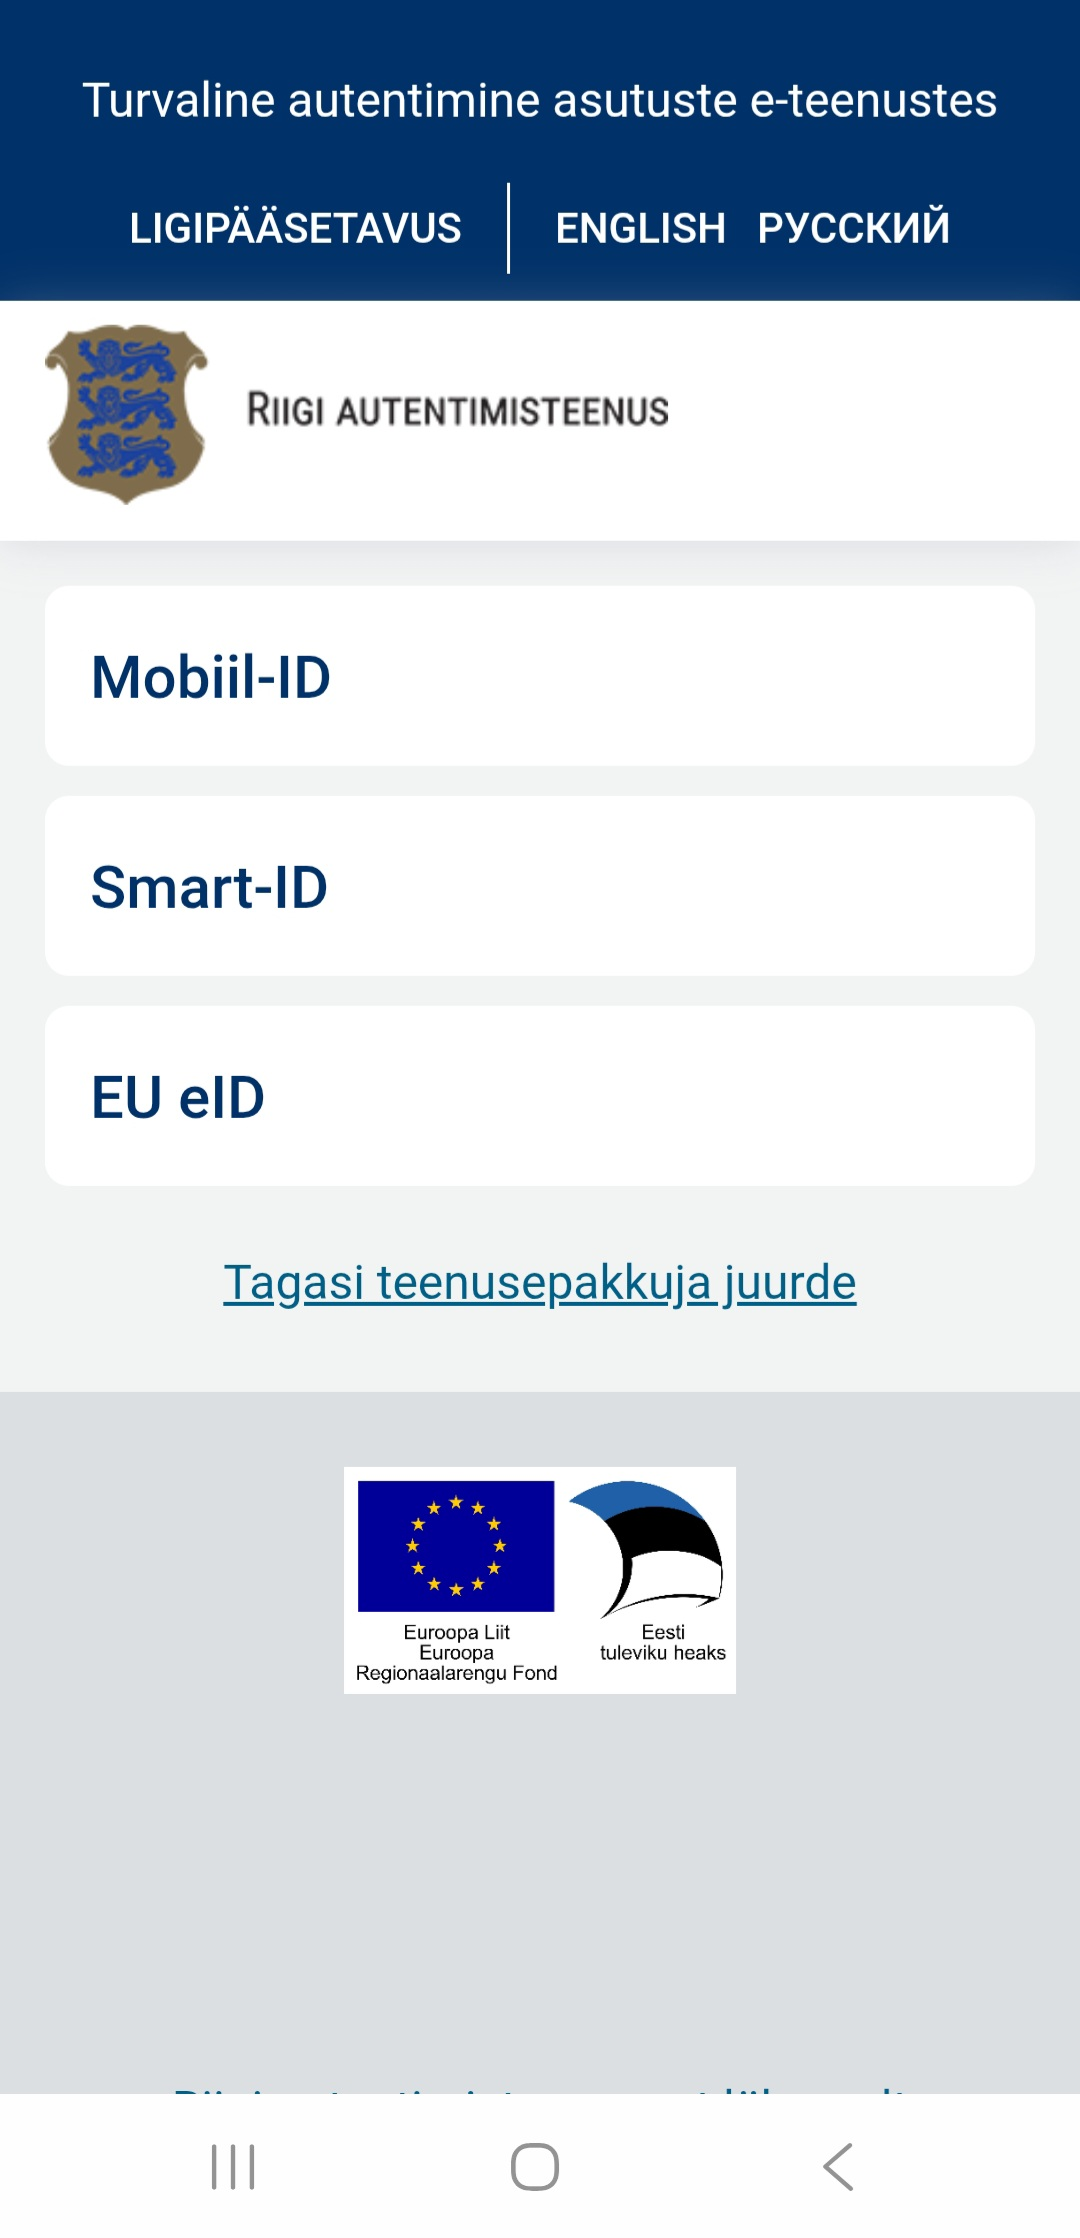
\includegraphics[width=0.3\textwidth]{../english/figures/Screenshot_20250812_212238_Data Access Notifier.jpg}
\end{center}
\end{column}
\end{columns}
\end{frame}

\begin{frame}
\frametitle{Key Implementation Challenges}
\begin{block}{Session Management}
\begin{itemize}
    \item Keeping the session alive (JWT token lives 30 minutes)
restriction
\end{itemize}
\end{block}

\begin{block}{Background Processing}
\begin{itemize}
    \item WorkManager: Unreliable for this use case due to system-managed delays
    \item Foreground Services: dataSync limited to 6 hours/day on Android 15+
    \begin{itemize}
        \item \textcolor{teal}{\textbf{Solution:}} Hybrid AlarmManager + Foreground service approach
    \end{itemize}
\end{itemize}
\end{block}

\begin{block}{Data Handling}
\begin{itemize}
    \item Filter self-queries (including queries to \textit{Andmejälgija} that also produce logs)
    \begin{itemize}
        \item \textcolor{teal}{\textbf{Solution:}} Filter 'receiver' by personal code.
    \end{itemize}
    \item Deduplication
    \begin{itemize}
        \item \textcolor{teal}{\textbf{Solution:}} Proto Data Store + Kotlin Set data structure.
    \end{itemize}
\end{itemize}
\end{block}
\end{frame}

\section{Results}

\begin{frame}
\frametitle{Implementation Results}
\begin{columns}
\begin{column}{0.6\textwidth}
\begin{itemize}
    \item \textbf{Platform:} Android 8.1+ (96.4\% coverage)
    \item \textbf{Language:} Kotlin
    \item \textbf{License:} MIT (Open Source)
    \item \textbf{Distribution:} GitHub Releases
    \item \textbf{Battery Impact:} Minimal
    \item \textbf{Tested Devices:}
    \begin{itemize}
        \item Xiaomi Poco X3 Pro (CrDroid)
        \item Xiaomi Redmi 7A (LineageOS)  
        \item Samsung Galaxy S25 (Stock)
    \end{itemize}
\end{itemize}
\end{column}
\begin{column}{0.4\textwidth}

\begin{center}

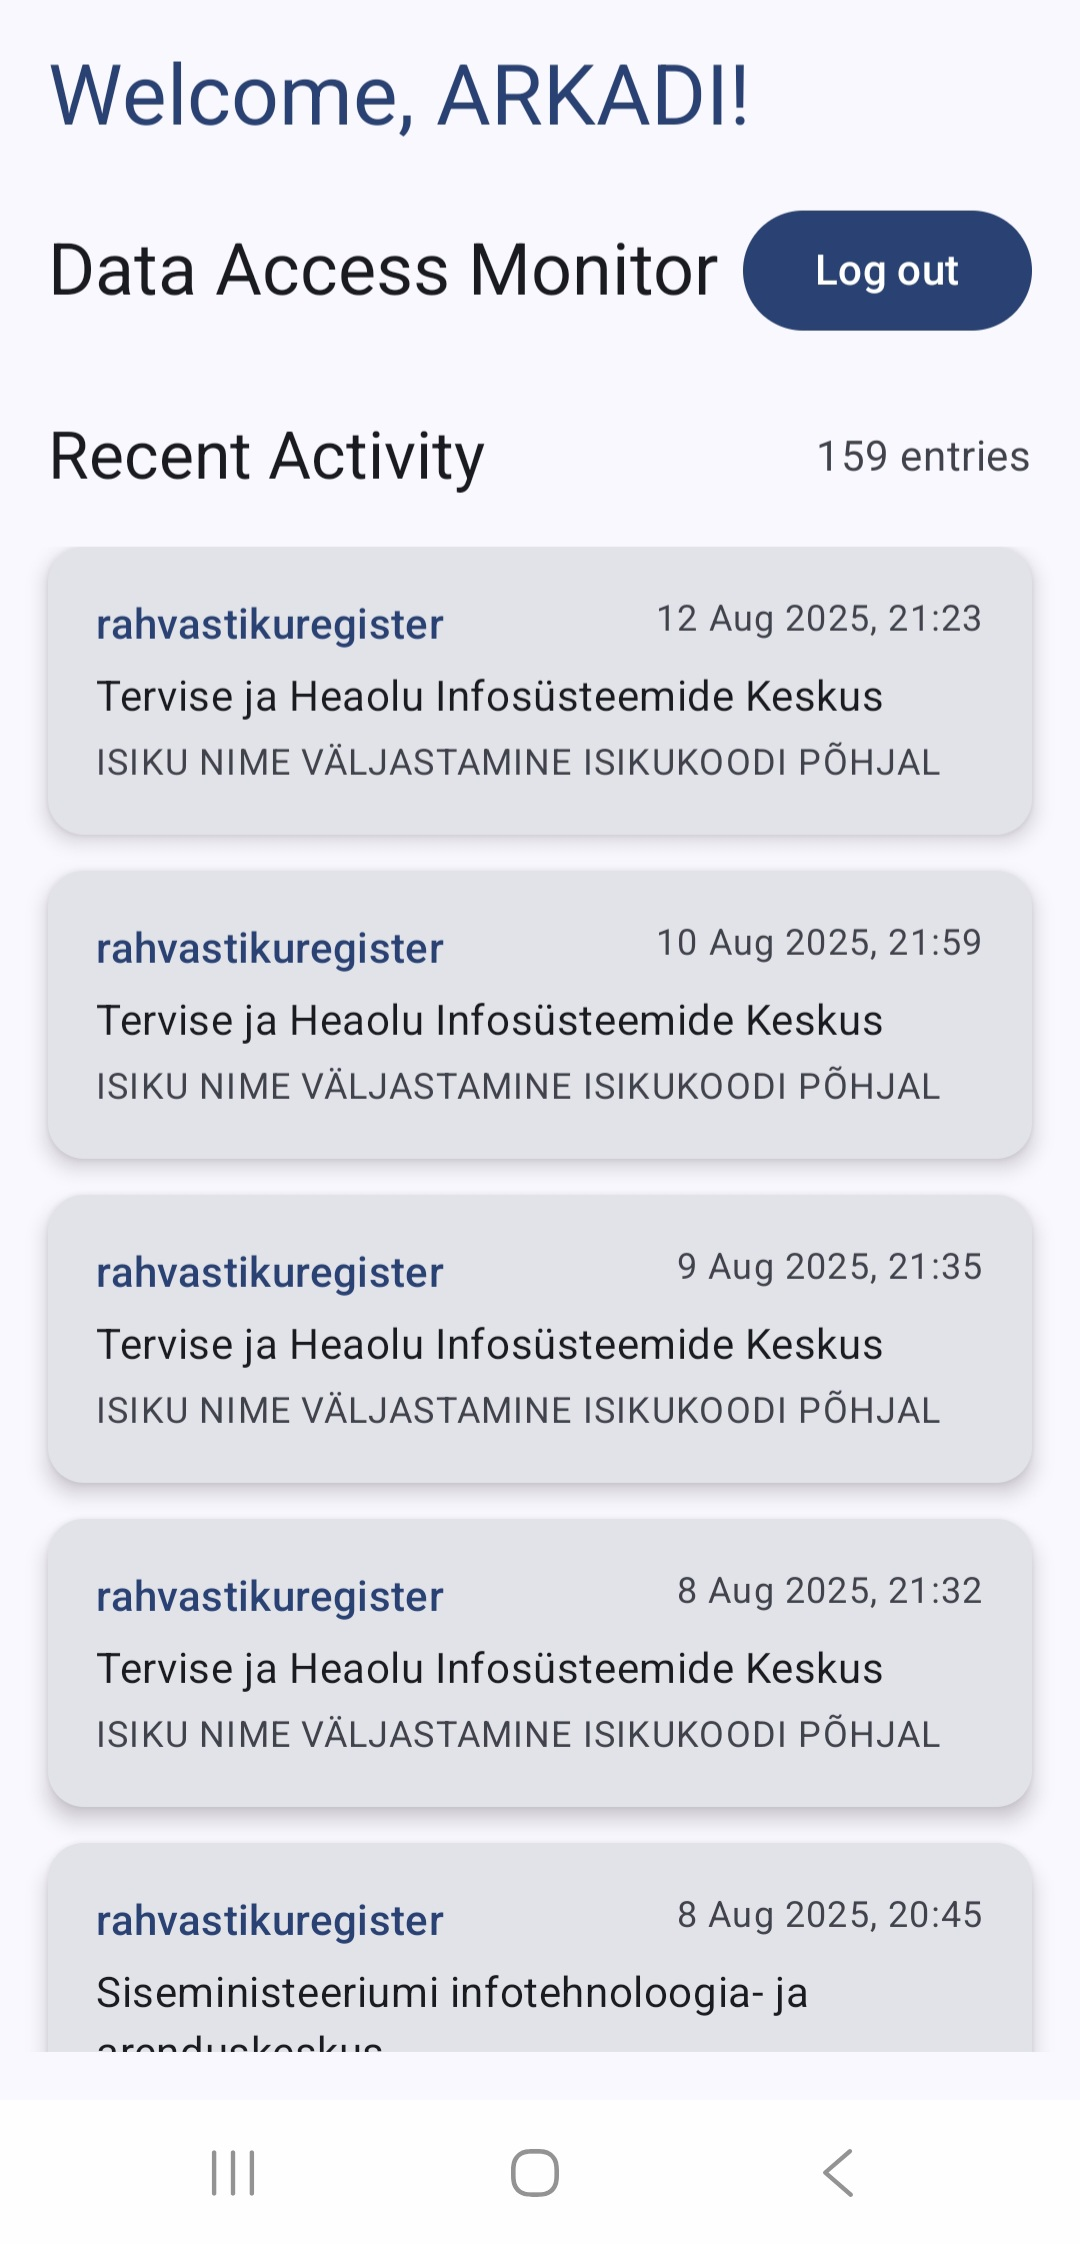
\includegraphics[width=0.55\textwidth]{../english/figures/Screenshot_20250812_212336_Data Access Notifier.jpg}
\end{center}
\end{column}
\end{columns}
\end{frame}

\begin{frame}
\frametitle{Implementation Results}
\begin{center}
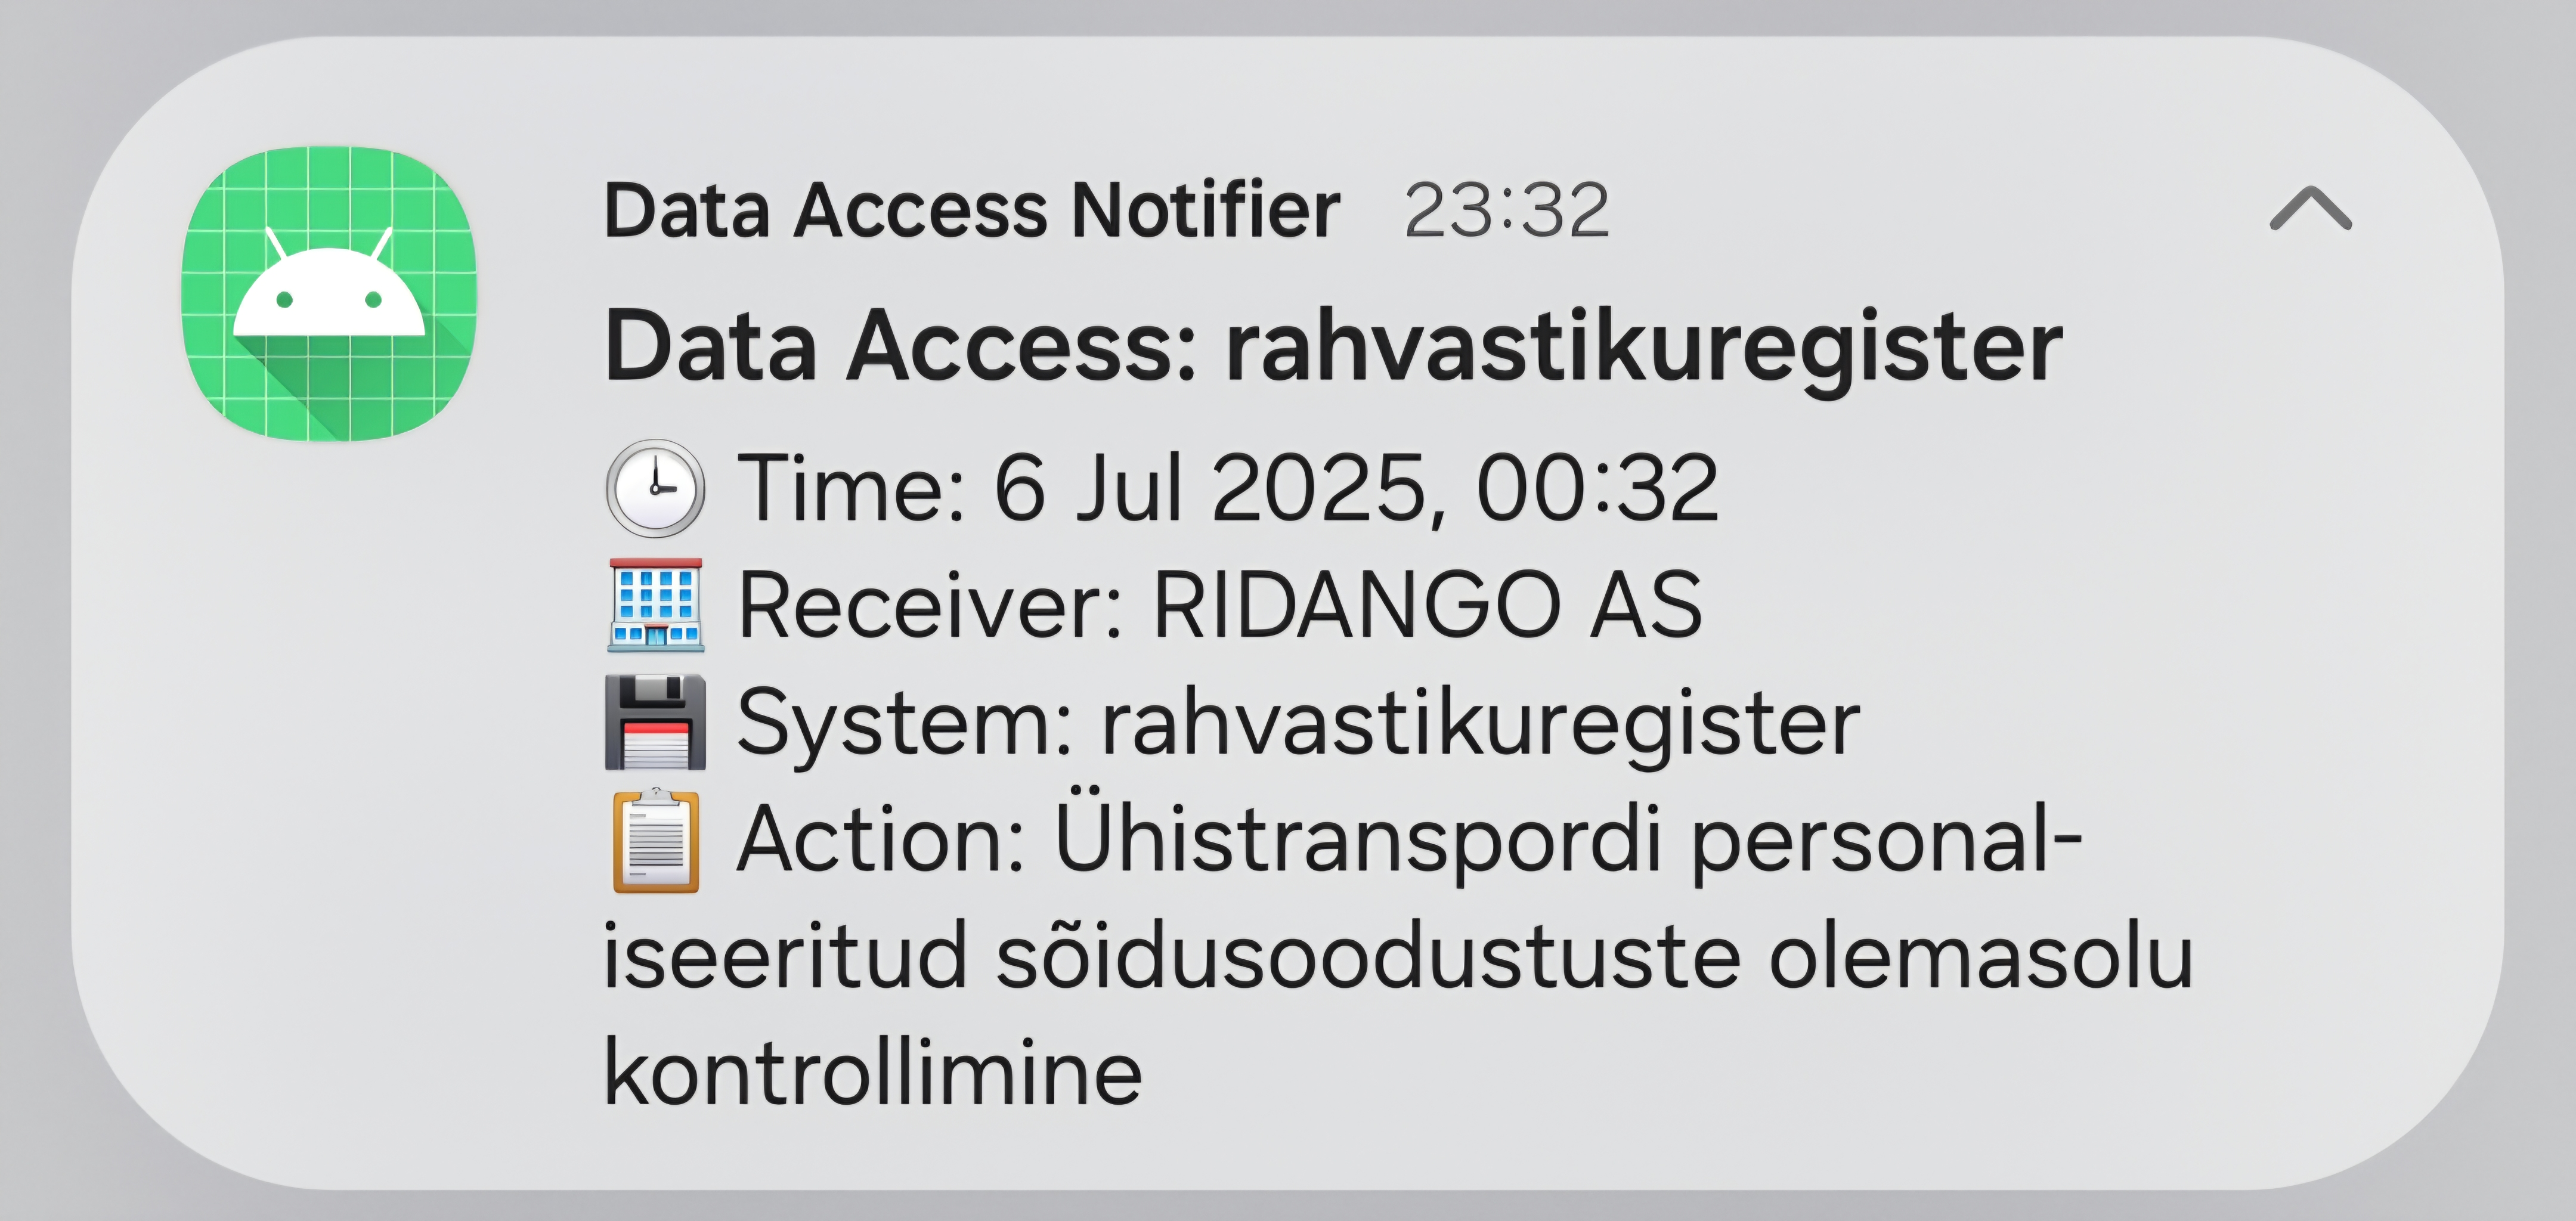
\includegraphics[width=0.8\textwidth]{../english/figures/IMG_20250812_233325_272.jpg}
\end{center}
\end{frame}

\begin{frame}
\frametitle{Key Observations During Testing}
\begin{block}{Delayed Log Entries}
\begin{itemize}
    \item Notifications received for events months in the past
    \begin{itemize}
        \item May 2025 (and even February 2025) events appearing in August 2025
        \item Suggests delays in logging infrastructure
    \end{itemize}
\end{itemize}
\end{block}

\begin{block}{Session Reliability}
\begin{itemize}
    \item AlarmManager + Foreground service approach highly reliable
    \begin{itemize}
        \item Successful operation even during extended device inactivity
        \item Maintains connectivity during network fluctuations
    \end{itemize}
\end{itemize}
\end{block}

% \begin{block}{User Experience}
% \begin{itemize}
%     \item Valuable insights into data access patterns
%     \item Transparency previously unavailable to users
%     \item Clear notifications about who accessed what data
% \end{itemize}
% \end{block}
\end{frame}

\section{Limitations}

\begin{frame}
\frametitle{Current Limitations}
\begin{block}{Technical Limitations}
\begin{itemize}
    \item \textcolor{red}{\textbf{12-hour session lifespan}} - hard server-side limit
    \item Android-only implementation
    \item Dependence on reverse-engineered API
\end{itemize}
\end{block}

\begin{block}{Coverage Limitations}
\begin{itemize}
    \item Limited to databases implementing \textit{Andmejälgija}
    \begin{itemize}
        \item Doesn't support E-File system
    \end{itemize}

\end{itemize}
\end{block}

\begin{itemize}
    \item Systematic issues
\end{itemize}

\end{frame}

\begin{frame}
\frametitle{Systematic Issues}
\begin{block}{Poor Quality Descriptions}
\begin{center}
\begin{tabular}{|p{3cm}|p{4cm}|}
\hline
\textbf{Bad Practice} & \textbf{Good Practice} \\
\hline
PERSONAL DATA BY PERSONAL CODE & Prescription viewed by doctor; prescription number 1018472350 \\
\hline
INDIVIDUAL EXTENDED INFO QUERY & Individual query for valid driver's licenses through state portal eesti.ee \\
\hline
\end{tabular}
\begin{tabular}{|p{2cm}|p{3cm}|}
\hline
\textbf{Bad Practice} & \textbf{Good Practice} \\
\hline
Doctor Viktor Pihlakas & INSTITUTION X \\
\hline
Jaan Kask 32405023456 & FOUNDATION Y \\
\hline
\end{tabular}
\end{center}
\end{block}

\begin{block}{Limited Coverage}
\begin{itemize}
    \item \textit{Andmejälgija} protocol is not legally mandated
    \begin{itemize}
        \item Even if database implements \textit{Andmejälgija}, not everything is necessarily logged.
    \end{itemize}
\end{itemize}
\end{block}
\end{frame}

% \begin{frame}
% \frametitle{Case Study: Missing Cross-Border Data Access}
% \begin{columns}
% \begin{column}{0.5\textwidth}
% \begin{block}{The Finnish Case}
% \begin{itemize}
%     \item Applied for criminal record extract from Finland
%     \item Finland requested my Estonian criminal record (May 14, 2025)
%     \item \textbf{No record} in Estonian E-File system from May 14-20
%     \item Finnish Legal Registry confirmed the request
% \end{itemize}
% \end{block}
% \end{column}
% \begin{column}{0.5\textwidth}
% \begin{center}
% 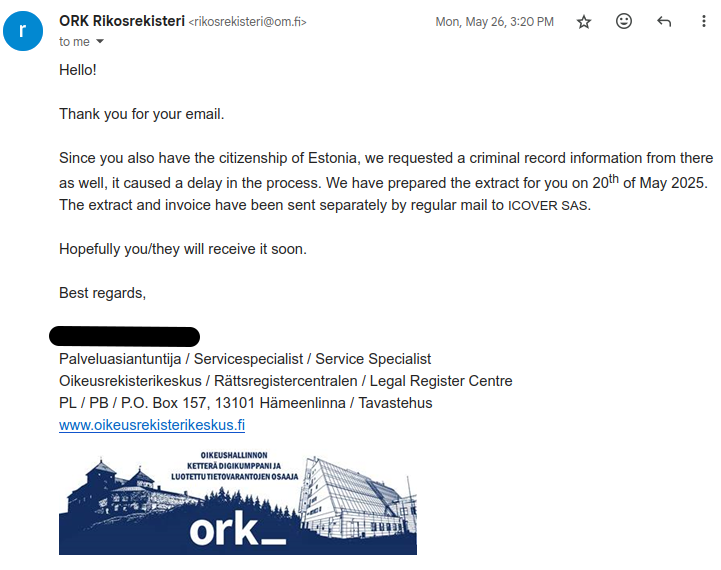
\includegraphics[width=\textwidth]{../english/figures/Screenshot from 2025-08-09 11-59-33.png}
% \end{center}
% \end{column}
% \end{columns}

% \end{frame}


% \begin{frame}
% \frametitle{Case Study: Missing Cross-Border Data Access}
% \begin{table}[H]
% \centering
% \begin{tiny}
% \begin{tabular}{|p{2.2cm}|p{4.2cm}|p{3.8cm}|p{2.3cm}|}
% \hline
% \textbf{Date} & \textbf{Query Type} & \textbf{Query Performer} & \textbf{Purpose} \\
% \hline
% 20.05.2025 & Query for all convictions (incl. archive data) & Arkadi Statsenko (E-File) & Person about themselves \\
% \hline
% 18.05.2025 & Query for all convictions & Defence Resources Agency, 70007647 (Conscripts Register) & Automatic control \\
% \hline
% 15.05.2025 & Query for all convictions (incl. archive data) & Arkadi Statsenko (E-File) & Person about themselves \\
% \hline
% 15.05.2025 & Query for all convictions (incl. archive data) & Arkadi Statsenko (E-File) & Person about themselves \\
% \hline
% 15.05.2025 & Query for all convictions (incl. archive data) & Arkadi Statsenko (E-File) & Person about themselves \\
% \hline
% \end{tabular}
% \end{tiny}
% \caption{\tiny E-File System query result showing the absence of cross-border data sharing records between 14.05.2025 and 20.05.2025}
% \label{tab:e-file-queries}
% \end{table}
% \end{frame}

% \section{Impact \& Significance}

% \begin{frame}
% \frametitle{Contributions \& Impact}
% \begin{block}{Technical Contribution}
% \begin{itemize}
%     \item Open source implementation available for community use
% \end{itemize}
% \end{block}

% \begin{block}{Policy Implications}
% \begin{itemize}
%     \item Demonstrates people's demand for data transparency
%     \item Highlights gaps in current tracking systems
% \end{itemize}
% \end{block}

% \begin{block}{Real-world Utility}
% \begin{itemize}
%     \item Provides previously unavailable real-time transparency
%     \item Enables proactive monitoring of personal data access
%     \item Catches delayed log entries that would be missed otherwise
% \end{itemize}
% \end{block}
% \end{frame}

\section{Conclusions}

\begin{frame}
\frametitle{Conclusions}
\begin{block}{Objectives Achieved}
\begin{itemize}
    \item \textcolor{teal}{\textbf{Done:}} Created functional mobile notification system
    \item \textcolor{teal}{\textbf{Done:}} Surveyed state database \textit{Andmejälgija} implementation
    \item \textcolor{teal}{\textbf{Done:}} Identified critical gaps in data access transparency
\end{itemize}
\end{block}

\begin{block}{Key Findings}
\begin{itemize}
    \item 12-hour GovSSO session limitation.
    \item Possible delays in logging
\end{itemize}
\end{block}

\begin{block}{Future Work}
\begin{itemize}
    \item Mitigation of 12-hour session constraint
    \item iOS/cross-platform implementation
    \item Getting listed on application stores (like Google Play)
\end{itemize}
\end{block}
\end{frame}

\begin{frame}
\frametitle{Thank You}
\begin{center}
\Large Questions?

\vspace{1cm}

\normalsize
\textbf{Data Access Notifier}\\
GitHub: \url{https://github.com/ArkadSt/DataAccessNotifier}

\vspace{0.5cm}

Contact: \href{mailto:arkadistatsenko@gmail.com}{arkadistatsenko@gmail.com}
\end{center}
\end{frame}

\begin{frame}
    \frametitle{Questions So Far}
    \begin{itemize}
        \item Why is Android 8.1 the minimum? Are there any libraries requiring Android 8.1 minimum?
        \item How long does it take to log in and view access logs in the app?
        \item Is it possible to forge JWT token to bypass eesti.ee API authentication checks?
        \item Which user's data is exactly accessed by an entity? Is it only personal identity code?
        \item What can users do after receiving a notification from the app?
    \end{itemize}
\end{frame}

\end{document}
